\documentclass[a4paper, 12pt]{article}
\usepackage{amsmath}
\usepackage{hyperref}
\usepackage{graphicx}
\usepackage{float}
\usepackage{booktabs}
\usepackage{tabularx}


\hypersetup{
	colorlinks=true,
	linkcolor=black
}

\begin{document}
	\pagenumbering{gobble}
	\begin{titlepage}
		\centering
		{\LARGE Controls Systems Practical 3 \par}
		\vspace*{1.5cm}
		{\large Q. Kruger, 216008466 \par}
		{\large R. de Bruyn, 216054484 \par}
		\vspace*{1.2cm}
		{\large \today}
		\vspace*{\fill}
		% 
\includegraphics[width=\textwidth]{img/UJ.jpg}
		\vspace*{\fill}
	\end{titlepage}

	\pagenumbering{roman}
	\tableofcontents
	\listoffigures
	\listoftables
	\newpage
	\pagenumbering{arabic}

	\section{Prelab} % (fold)
	\label{sec:prelab}
		\subsection{Question 1} % (fold)
		\label{sub:prelab_question_1}
			The settling time for a first order transfer function of the form
			\[
				G(s) = \frac{a}{s + a}
			\]
			is given by the formula
			\begin{equation}
				T_s(a) = \frac{4}{a}
				\label{eq:settle}
			\end{equation}
			and the rise time for the same transfer function is given by
			\begin{equation}
				T_r(a) = \frac{2.2}{a}
				\label{eq:rise_1st}
			\end{equation}
			Using \eqref{eq:settle} and \eqref{eq:rise_1st}, we can easily find the settling time and rise time in seconds. Here follows the poles time response values for various values of $a$
			\[
				T_s(1) = 4\,\text{s}
			\]
			\[
				T_r(1) = 2.2\,\text{s}
			\]
			\begin{figure}[H]
				\centering
				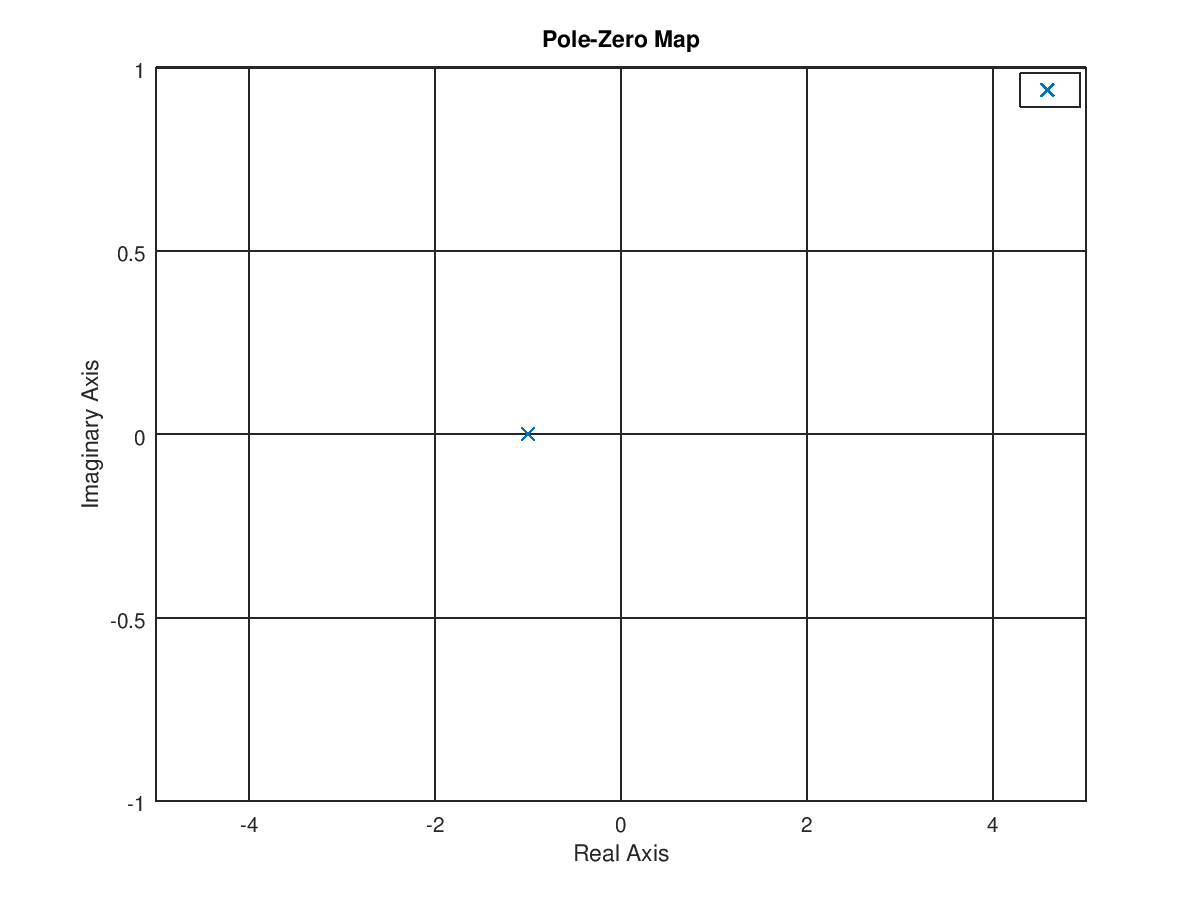
\includegraphics[width=0.7\textwidth]{img/1st1.png}
				\caption{Pole plot for $a = 1$}
				\label{fig:1}
			\end{figure}
			\[
				T_s(2) = 2\,\text{s}
			\]
			\[
				T_r(2) = 1.1\,\text{s}
			\]
			
			\begin{figure}[H]
				\centering
				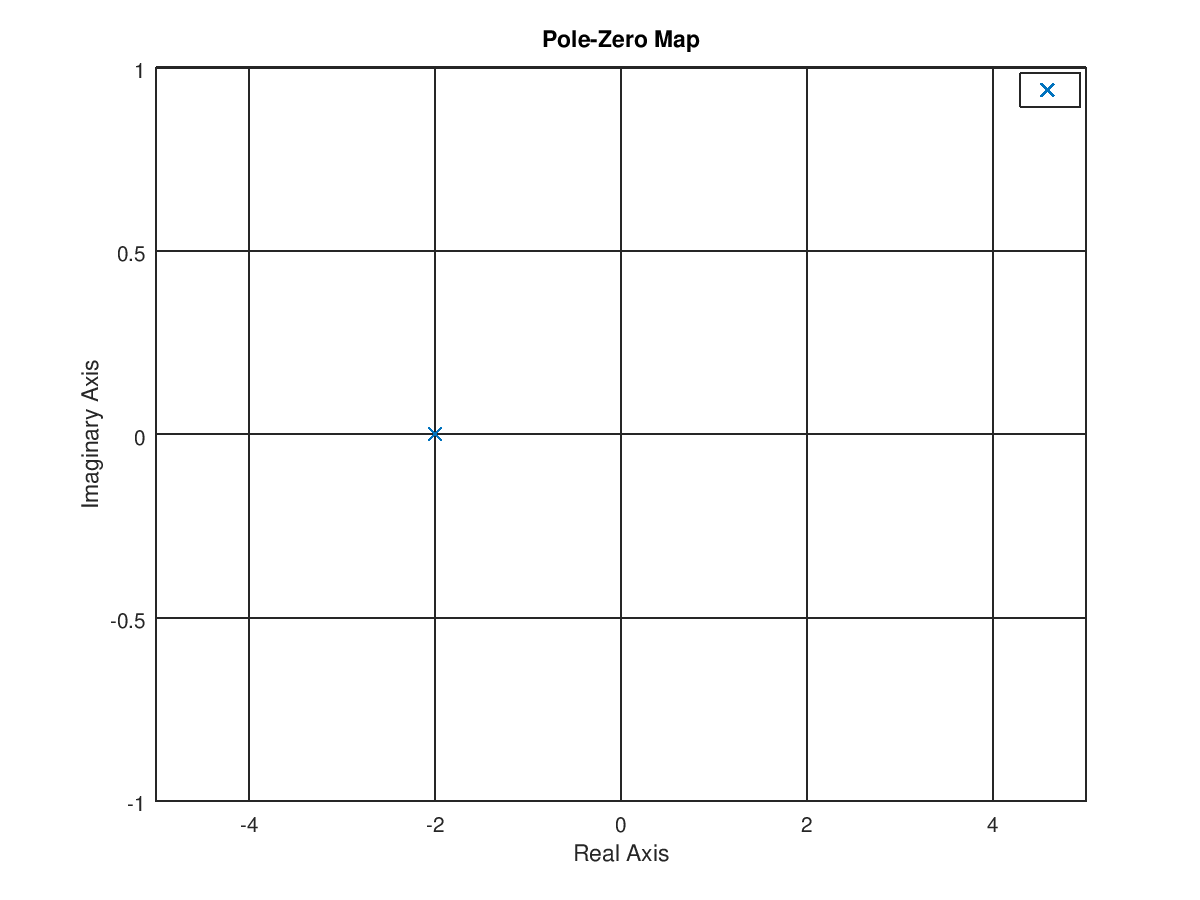
\includegraphics[width=0.7\textwidth]{img/1st_2.png}
				\caption{Pole plot for $a = 2$}
				\label{fig:1}
			\end{figure}
			\[
				T_s(3) = \frac{4}{3} \approx 1.33\,\text{s}
			\]
			\[
				T_r(3) = \frac{2.2}{3} = 0.73\,\text{s}
			\]

			\begin{figure}[H]
				\centering
				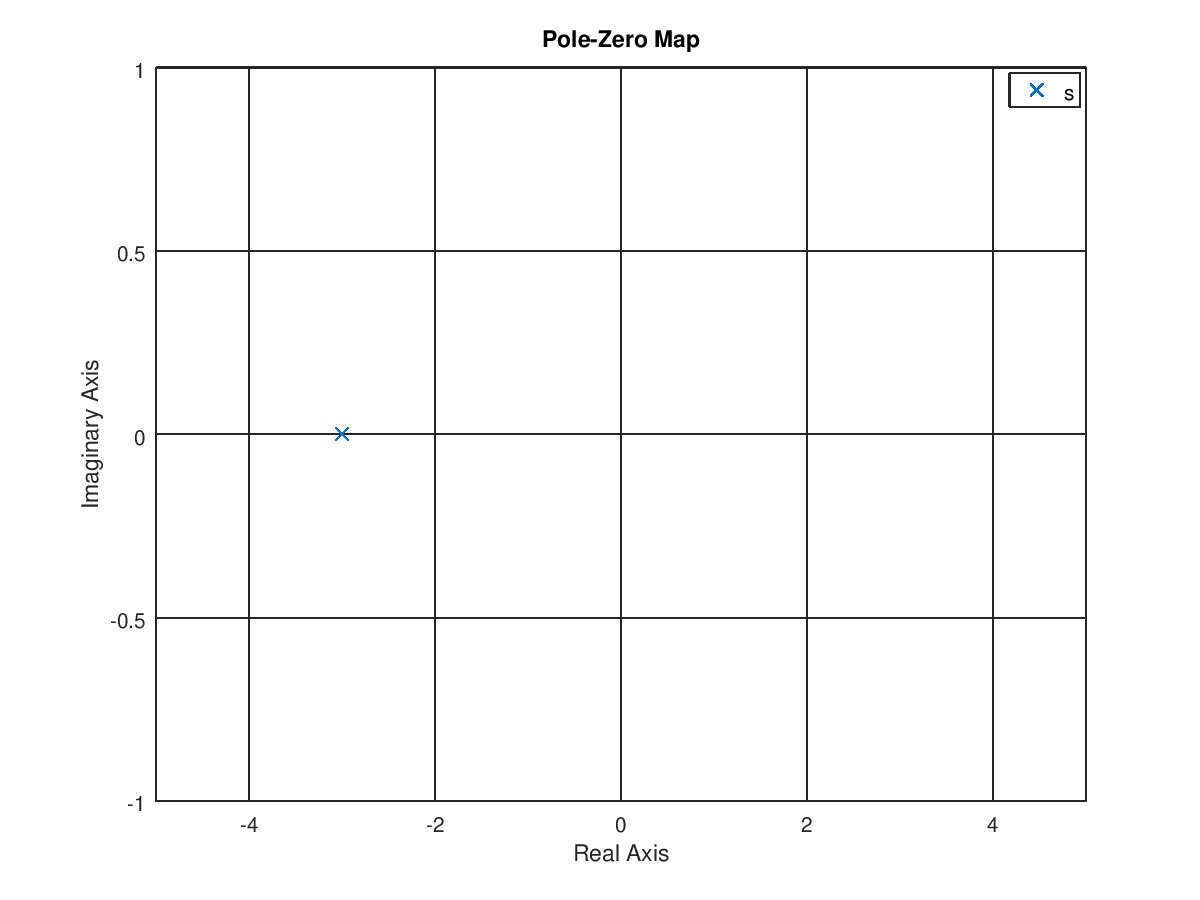
\includegraphics[width=0.7\textwidth]{img/1st_3.png}
				\caption{Pole plot for $a = 3$}
				\label{fig:1}
			\end{figure}
		% subsection prelab_question_1 (end)

		\subsection{Question 2} % (fold)
		\label{sub:prelab_question_2}
			For this question, we will investigate how the time response of second order systems changes when the real and imaginary components of the poles are altered. The equation for the components of a pole are given by
			\begin{equation}
				\begin{array}{rcl}
					s & = & -\zeta\omega_n \pm j\omega_n\sqrt{1 - \zeta^2} \\
					& = & -\sigma_d \pm j\omega_d
				\end{array}
				\label{eq:pole_exp}
			\end{equation}
			and the parameters relating to its time response are
			\begin{equation}
				T_s(\sigma_d) = \frac{4}{\sigma_d}
				\label{eq:2nd_ts}
			\end{equation}
			\begin{equation}
				T_p(\omega_d) = \frac{\pi}{\omega_d}
				\label{eq:2nd_tp}
			\end{equation}
			\begin{equation}
				T_r(\omega_n, \zeta) = \tfrac{1}{\omega_n}(1.76\zeta^3 - 0.417\zeta^2 + 1.039 \zeta + 1)
				\label{eq:2nd_tr}
			\end{equation}
			\begin{equation}
				\%OS(\zeta) = \exp\left(-\frac{\zeta\pi}{\sqrt{1 - \zeta^2}}\right) \times 100
				\label{eq:2nd_os}
			\end{equation}

			Since the real and imaginary components are both dependent on $\zeta$ and $\omega_n$, we have to derive a formula to leave the imaginary part of a pole the same after altering the aforementioned parameters, but alter the real part by some factor. Letting this factor be $K$, we can write the system of equations that govern this change as
			\begin{equation}
				\begin{array}{rcl}
					\omega_d' & = & \omega_d \\
					\omega_n'\sqrt{1 - \zeta'^2} & = & \omega_n\sqrt{1 - \zeta^2}
				\end{array}
				\label{eq:der_1}
			\end{equation}
			and
			\begin{equation}
				\begin{array}{rcl}
					\sigma_d' & = & K\sigma_d \\
					\zeta'\omega_n' & = & K \zeta\omega_n
				\end{array}
				\label{eq:der_2}
			\end{equation}

			By substituting $\omega_n' = \frac{K\zeta\omega_n}{\zeta'}$, derived from \eqref{eq:der_2}, into \eqref{eq:der_1}, we get
			\begin{equation}
				\begin{array}{rcl}
					K\zeta\omega_n \frac{\sqrt{1 - \zeta'^2}}{\zeta'} & = & \omega_n\sqrt{1 - \zeta^2} \\
					K\zeta \frac{\sqrt{1 - \zeta'^2}}{\zeta'} & = & \sqrt{1 - \zeta^2} \\
					\frac{\sqrt{1 - \zeta'^2}}{\zeta'} & = & \frac{\sqrt{1 - \zeta^2}}{K\zeta} \\
					\frac{1 - \zeta'^2}{\zeta'^2} & = & \frac{1 - \zeta^2}{K^2\zeta^2} \\
					1 - \zeta'^2 & = & \left(\frac{1 - \zeta^2}{K^2\zeta^2}\right)\zeta'^2 \\
					\left(\frac{1 - \zeta^2}{K^2\zeta^2} + 1\right) \zeta'^2 & = & 1 \\
					\left(\frac{1 + (K^2 - 1) \zeta^2}{K^2\zeta^2}\right) \zeta'^2 & = & 1 \\
					\zeta' & = & \sqrt{\frac{K^2\zeta^2}{1 + (K^2 - 1) \zeta^2}} \\
					\zeta' & = & \frac{K\zeta}{\sqrt{1 + (K^2 - 1) \zeta^2}} \\
				\end{array}
				\label{eq:zeta_dash}
			\end{equation}
			and substituting this expression from \eqref{eq:zeta_dash} into \eqref{eq:der_2}, we get
			\begin{equation}
				\begin{array}{rcl}
					\omega_n' & = & \frac{K \zeta \omega_n}{\zeta'} \\
					& = & K\zeta\omega_n\frac{\sqrt{1 + (K^2 - 1)\zeta^2}}{K\zeta} \\
					& = & \omega_n\sqrt{1 + (K^2 - 1)\zeta^2}
				\end{array}
				\label{eq:omega_dash}
			\end{equation}

			Now, if we consider the equation for a second order transfer function given by
			\[
				G(s) = \frac{\omega_n^2}{s^2 + 2\omega_n\zeta + \omega_n^2} = \frac{25}{s^2 + 4s + 25}
			\]
			we can easily calculate that $\omega_n = 5$ and $\zeta = \frac{2}{5}$, and thus that $\sigma_d = 2$ and $\omega_d = \sqrt{21}$. From this transfer function, then, the time response is
			\[
				\%OS = 25.38\%
			\]

			\[
				T_s = 2 \,\text{s}
			\]

			\[
				T_p = 0.6856\,\text{s}
			\]

			\[
				T_r = 0.2923\,\text{s}
			\]

			Multiplying the real part of the poles of $G(s)$ with a factor of $K=2$, we use formulas \eqref{eq:zeta_dash} and \eqref{eq:omega_dash} to find our new parameters, denoted $\omega_n' = \sqrt{37}$, $\zeta' = \frac{4}{\sqrt{37}}$, $\sigma_d' = 4$, and $\omega_d' = \omega_d = \sqrt{21}$. Our modified time response to multiplying the real part of the pole by 2 is

			\[
				\%OS' = 6.44\%
			\]

			\[
				T_s' = 1\,\text{s}
			\]

			\[
				T_p' = 0.6856\,\text{s}
			\]

			\[
				T_r' = 0.3294\,\text{s}
			\]

			Using the same process as above, multiplying the real part of the poles of $G(s)$ with a factor of $K=\frac{1}{2}$, we get $\omega_n'' = \sqrt{22}$, $\zeta'' = \frac{1}{\sqrt{22}}$, $\sigma_d'' = 1$, and $\omega_d'' = \omega_d = \sqrt{21}$. Our modified time response in this case is

			\[
				\%OS'' = 50.38\%
			\]

			\[
				T_s'' = 4\,\text{s}
			\]

			\[
				T_p'' = 0.6856\,\text{s}
			\]

			\[
				T_r'' = 0.26\,\text{s}
			\]

		% subsection prelab_question_2 (end)
	% section prelab (end)

	\section{Lab} % (fold)
	\label{sec:lab}
		This experiments was done using the Ocatve Control package
	\subsection{Question 1}
	\label{sec:question_1_lab}
		The transfer functions of interest in this Lab question are:
			\begin{equation*}
				\begin{array}{rcl}
					g_1 = \frac{1}{s+1}\\
					g_2 = \frac{2}{s+2}\\
					g_3 = \frac{3}{s+3}
				\end{array}
			\end{equation*}
		$g_1$, $g_2$ and $g_3$ were captured in an Octave function and the step responses of these systems were obtained by executing the function given as:\par
		\texttt{g1 = tf([1],[1,1])}\par
		\texttt{g2 = tf([2],[1,2])}\par
		\texttt{g3 = tf([3],[1,3])}\par

		\texttt{step(g1, 'r');}\par
		\texttt{hold on;}\par
		\texttt{step(g2, 'g');}\par
		\texttt{hold on;}\par
		\texttt{step(g3, 'b');}\par
		\texttt{hold off;}\par

		\texttt{legend('g1','g2','g3');}\par

		The plot obtained for this function is given in Figure \ref{fig:plot_question_1_lab} which shows the step responses of the respective systems:

		\begin{figure}[H]
			\centering
			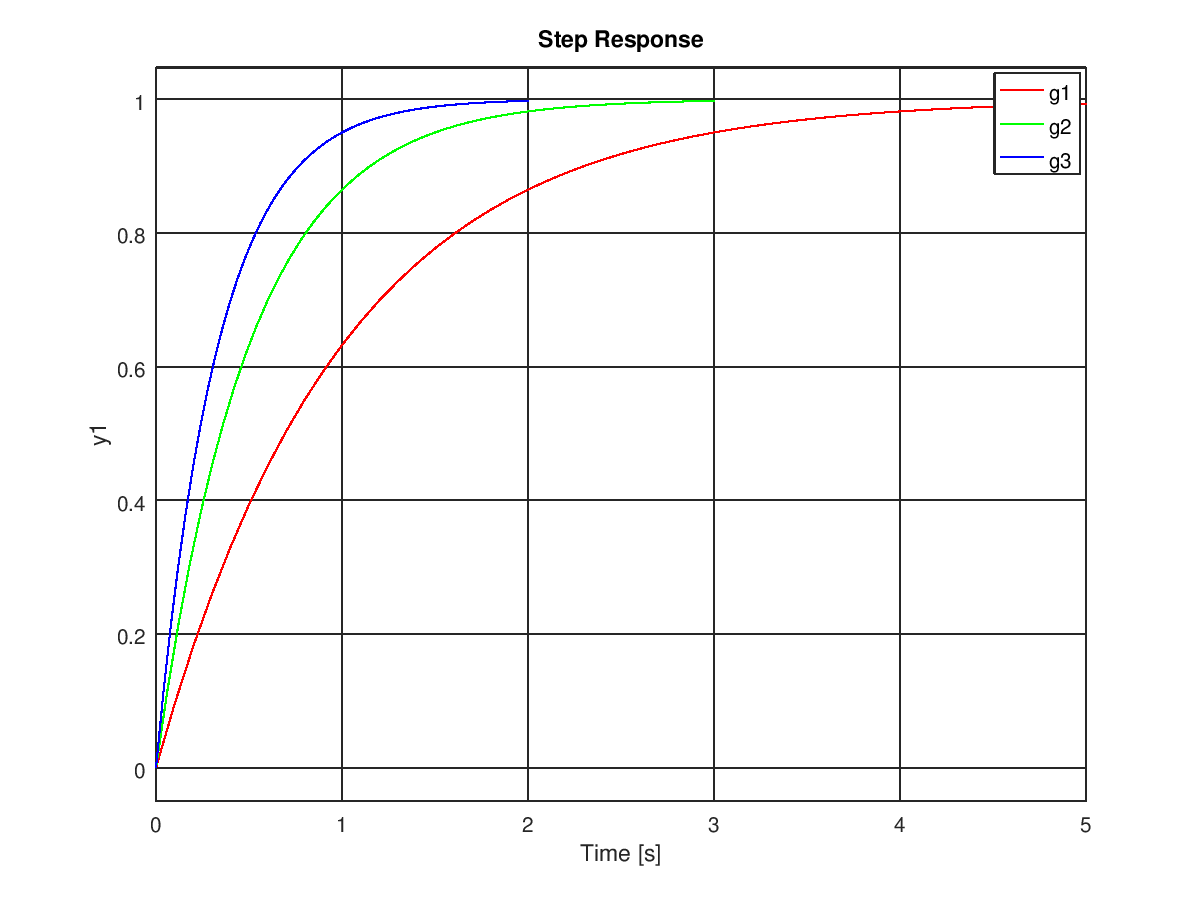
\includegraphics[width = 150mm]{img/Question_1_Lab_Plots.png}
			\caption{Step reponse plots for the different systems described by respective transfer functions}
			\label{fig:plot_question_1_lab}
		\end{figure}

		\textit{stepinfo function equicvalent in octave to give rise- and settling time}

	\subsection{Question 2}
	\label{question_2_lab}
		The transfer function relevant to the discussion of this Lab experiment is given as:
		\begin{equation}
				G(s) = \frac{b}{s^2+as+b}	
		\end{equation}

		Substituting in values for \texttt{a} and \texttt{b} given as $a = 4$ and $b = 25$ gives the transfer function \texttt{G\_1}:
		\begin{equation}
			G_1(s) = \frac{25}{s^2+4s+25}\\
		\end{equation}

		The poles of this transfer function is given as 
		\begin{equation}
			\begin{array}{rcl}
				s_1 = -4 + i\sqrt{21}\\
				s_2 = -4 - i\sqrt{21}\\
			\end{array}
		\end{equation}

		Finding the values of \texttt{a} and \texttt{b} for changed real components of the poles where the first change is two times the real pole components of the system described by the transfer function \texttt{G\_1}. The values of \texttt{a} and \texttt{b} are given as $a = 8$ and $b = 37$. Thus the new transfer function is given as:

		\begin{equation}
			G_2(s) = \frac{37}{s^2+8s+37}\\
		\end{equation}

		The values of \texttt{a} and \texttt{b} for the real components of the poles of the system described by \texttt{G\_1} halved is $a = 2$ and $b = 22$. The resulting transfer function is given as:
		\begin{equation}
			G_3(s) = \frac{22}{s^2+2s+22}\\
		\end{equation}

		Finding the step response of these transfer functions (\texttt{G\_1, G\_2 and G\_3}) by running the following code in Octave:

		\texttt{g1 = tf([25],[1 4 25]);}\par
		\texttt{g2 = tf([37],[1 8 37]);}\par
		\texttt{g3 = tf([22],[1 2 22]);}\par

		\texttt{step(g1, 'r');}\par
		\texttt{hold on;}\par
		\texttt{step(g2, 'g');}\par
		\texttt{hold on;}\par
		\texttt{step(g3, 'b');}\par
		\texttt{hold off;}\par

		\texttt{legend('g1','g2','g3')}



		gives a plot as shown in Figure \ref{plot_question_2_lab}:

		\begin{figure}[H]
			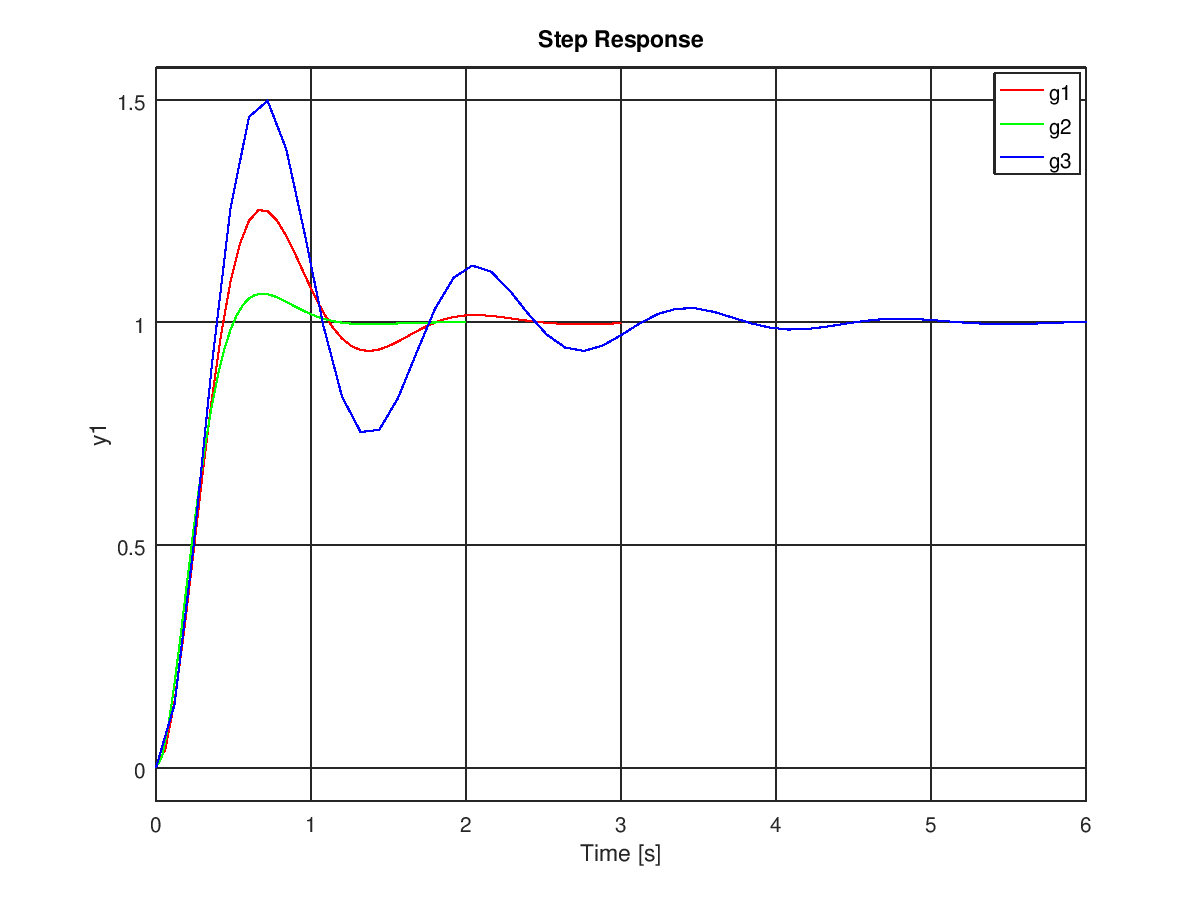
\includegraphics[width=\textwidth]{img/Question_2_Lab_Plots.png}
			\caption{Step response plots for the different systems described by respective transfer functions}
			\label{plot_question_2_lab}
		\end{figure}

		\subsection{Stepinfo calculation} % (fold)
		\label{sub:stepinfo_calculation}
			We used the \texttt{stepinfo} function from Matlab in order to calculate the time response parameters for the second and first order systems. For the sake of brevity, the results have been tabulated for comparison in Table \ref{table:1st} and Table \ref{table:2nd} respectively.
		% subsection stepinfo_calculation (end)

	% section lab (end)

	\section{Postlab} % (fold)
	\label{sec:postlab}
		\begin{table}[H]
			\begin{tabularx}{\textwidth}{X X X X X X}
				\toprule
				\multicolumn{2}{X}{$a$} & \multicolumn{2}{X}{$T_r$} & \multicolumn{2}{X}{$T_s$} \\
				& & Exp. & Thr. & Exp. & Thr. \\
				\midrule
				1 & & 2.2 & 2.2 & 4 & 4 \\
				2 & & 1.1 & 1.1 & 2 & 2 \\
				3 & & 0.73 & 0.73 & 1.33 & 1.33 \\
				\bottomrule
			\end{tabularx}
			\caption{Time response properties for different pole positions of first order systems}
			\label{table:1st}
		\end{table}

		\begin{table}[H]
			\begin{tabularx}{\textwidth}{X X X X X X X X X X X X}
			\toprule
			\multicolumn{2}{X}{$\omega_d$} & \multicolumn{2}{X}{$\sigma_d$} & \multicolumn{2}{X}{$T_r$} & \multicolumn{2}{X}{$T_p$} & \multicolumn{2}{X}{$T_s$} & \multicolumn{2}{X}{$\%OS$} \\
			 & & & & Exp & Thr & Exp & Thr & Exp & Thr & Exp & Thr \\
			\midrule
			$\sqrt{21}$ & & 2 & & 0.292 & 0.292 & 0.686 & 0.686 & 2 & 2 & 25.38 & 25.38 \\
			$\sqrt{21}$ & & 4 & & 0.329 & 0.329 & 0.686 & 0.686 & 1 & 1 & 6.44 & 6.44 \\
			$\sqrt{21}$ & & 1 & & 0.260 & 0.260 & 0.686 & 0.686 & 4 & 4 & 50.38 & 50.38 \\
			\bottomrule
			\end{tabularx}
			\caption{Time response properties for different pole positions for second order systems}
			\label{table:2nd}
		\end{table}

		Looking at the values in Table \ref{table:1st} and Table \ref{table:2nd}, we can see that the experimental values for the first and second order systems are very close to the theoretical values that were calculated using the formulae in the Prelab. We can thus conclude that the theoretical expectations are met by the experimental results, and that the theory is valid.
	% section postlab (end)

\end{document}